\documentclass[../../main.tex]{subfiles}
\begin{document}

\begin{flushright}
  \footnotesize\textit{【自動文字起こし・要確認】}
\end{flushright}

［解］$y = 4 - x^2$ 上の $x = t$ での接線 $l$ は ($0 < t < 2$)
\begin{align}
  l: y = f(x) = -2tx + 4 + t^2
\end{align}
だからこれが $(a, 0)$ を通る時，
\begin{align}
  0 = t^2 - 2at + 4
\end{align}
\begin{align}
  \therefore t = a - \sqrt{a^2 - 4} \quad (\because t < 2, a > 2)
\end{align}
である．これを $t_0$ とおくと，図から

\begin{figure}[htb]
  \centering
  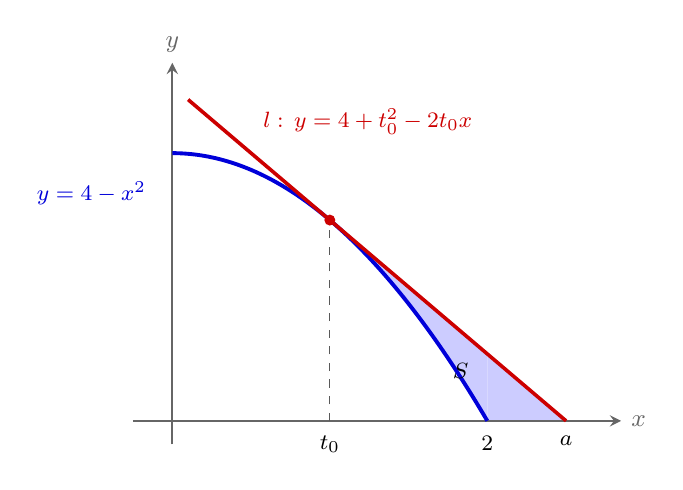
\begin{tikzpicture}[x=2.0cm, y=0.85cm, >=stealth,
    every node/.style={font=\small}]
    % Illustrative a=5/2 gives t_0=1 and l: y=5-2x.
    \fill[blue!20] (1,3)
    -- plot[domain=1:2, samples=40] (\x,{5-2*\x})
    -- (2,0)
    -- plot[domain=2:1, samples=40] (\x,{4-\x*\x}) -- cycle;
    \fill[blue!20] (2,0) -- (2,1) -- (2.5,0) -- cycle;
    \draw[->, thick, gray!80!black] (-0.25,0) -- (2.85,0) node[right] {$x$};
    \draw[->, thick, gray!80!black] (0,-0.35) -- (0,5.35) node[above] {$y$};
    \draw[line width=1.4pt, blue!85!black, domain=0:2,
    samples=80, smooth] plot (\x,{4-\x*\x});
    \draw[line width=1.3pt, red!80!black] (0.1,4.8) -- (2.5,0);
    \draw[dashed, gray!70!black] (1,0) -- (1,3);
    \node[circle, fill=red!80!black, inner sep=1.4pt] at (1,3) {};
    \node[above right=2pt, red!80!black, font=\footnotesize] at (0.48,4.05)
    {$l:\,y=4+t_0^2-2t_0x$};
    \node[left=6pt, blue!85!black, font=\footnotesize] at (0,3.4)
    {$y=4-x^2$};
    \node[font=\footnotesize] at (1.83,0.75) {$S$};
    \node[below=2pt, font=\footnotesize] at (1,0) {$t_0$};
    \node[below=2pt, font=\footnotesize] at (2,0) {$2$};
    \node[below=2pt, font=\footnotesize] at (2.5,0) {$a$};
  \end{tikzpicture}
  \caption{放物線・接線・$x$ 軸で囲まれる領域 $S$}
  \label{fig:1962_6_area}
\end{figure}

求める面積 $S$ は
\begin{align}
  S &= \int_{t_0}^2 (f(x) - (4-x^2)) dx + \dfrac{1}{2} (a-2)^2 \cdot 2t_0 \\
  &= \int_{t_0}^2 (x - t_0)^2 dx + t_0 (a-2)^2 \\
  &= \dfrac{1}{3} (2 - t_0)^3 + t_0 (a-2)^2
\end{align}
（$A = \sqrt{2+a}, B = \sqrt{a-2}$ とおく）
\begin{align}
  &= \dfrac{1}{3} (-B^2 + AB)^3 + (a - AB) B^4 \\
  &= \dfrac{1}{3} B^3 (A^3 - 3A^2 B + 3AB^2 - B^3) + aB^4 - AB^5 \\
  &= \dfrac{1}{3} B^3 (A^3 - B^3) - A^2 B^4 + aB^4 \\
  &= \dfrac{1}{3} \left( (a^2-4)^{\frac{3}{2}} - (a-2)^3 \right) - 2(a-2)^2 \\
  &= \dfrac{1}{3} (a^2-4)^{\frac{3}{2}} - \dfrac{1}{3} (a+4)(a-2)^2
\end{align}

\begin{framed}
  思ったより大変だった．他の方法だと...

  \begin{align}
    S &= \text{台形} - \triangle \\
    &= \dfrac{1}{2} (a-t_0)^2 \cdot 2t_0 - \int_{t_0}^2 (4-x^2) dx \\
    &= t_0 (a^2-4) - \dfrac{16}{3} + 4t_0 - \dfrac{1}{3} t_0^3 \\
    &= t_0 \left( 4 - \dfrac{1}{3} t_0^2 + a^2-4 \right) - \dfrac{16}{3} \\
    &= \dfrac{1}{3} (a - \sqrt{a^2-4}) \left( a^2 + 4 + 2a\sqrt{a^2-4} \right) - \dfrac{16}{3} \\
    &= \dfrac{1}{3} \left[ a(a^2+4) - 20(a^2-4) + (a^2-4)^{\frac{3}{2}} \right] - \dfrac{16}{3} \\
    &= \dfrac{1}{3}(a^2-4)^{\frac{3}{2}} - \dfrac{1}{3}(a+4)(a-2)^2
  \end{align}
\end{framed}

\end{document}
